\section{Relational Model}

\begin{figure}[ht]
    \centering
    \makebox[\textwidth][c]{
    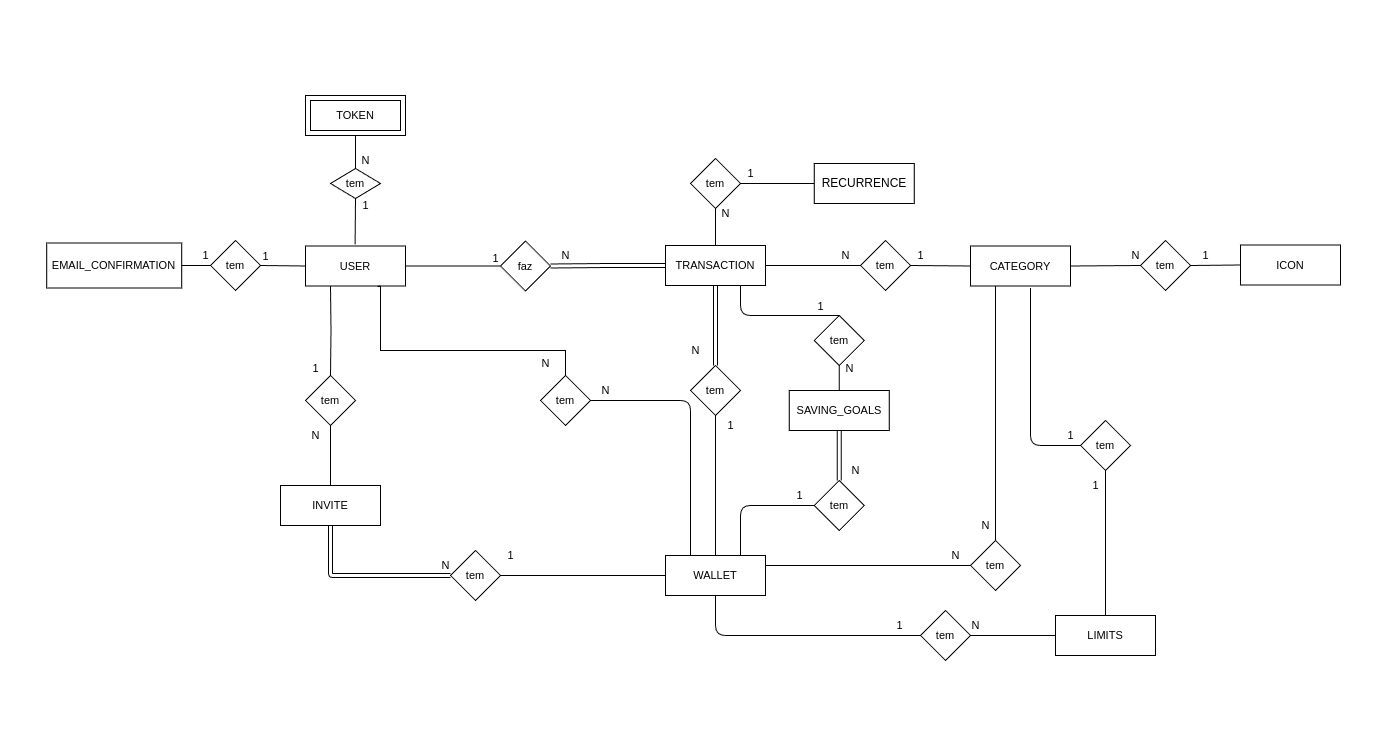
\includegraphics[width=1.3\textwidth]{./img/SimpleERModel.png}
    }
    \caption{Database Structure without attributes, Check complete ER Model on Appendix \ref{fig:er_model}}
    \label{fig:database_structure}
\end{figure}

\begin{figure}[H]
    \centering
    \begin{subfigure}[b]{\textwidth}
        \centering
        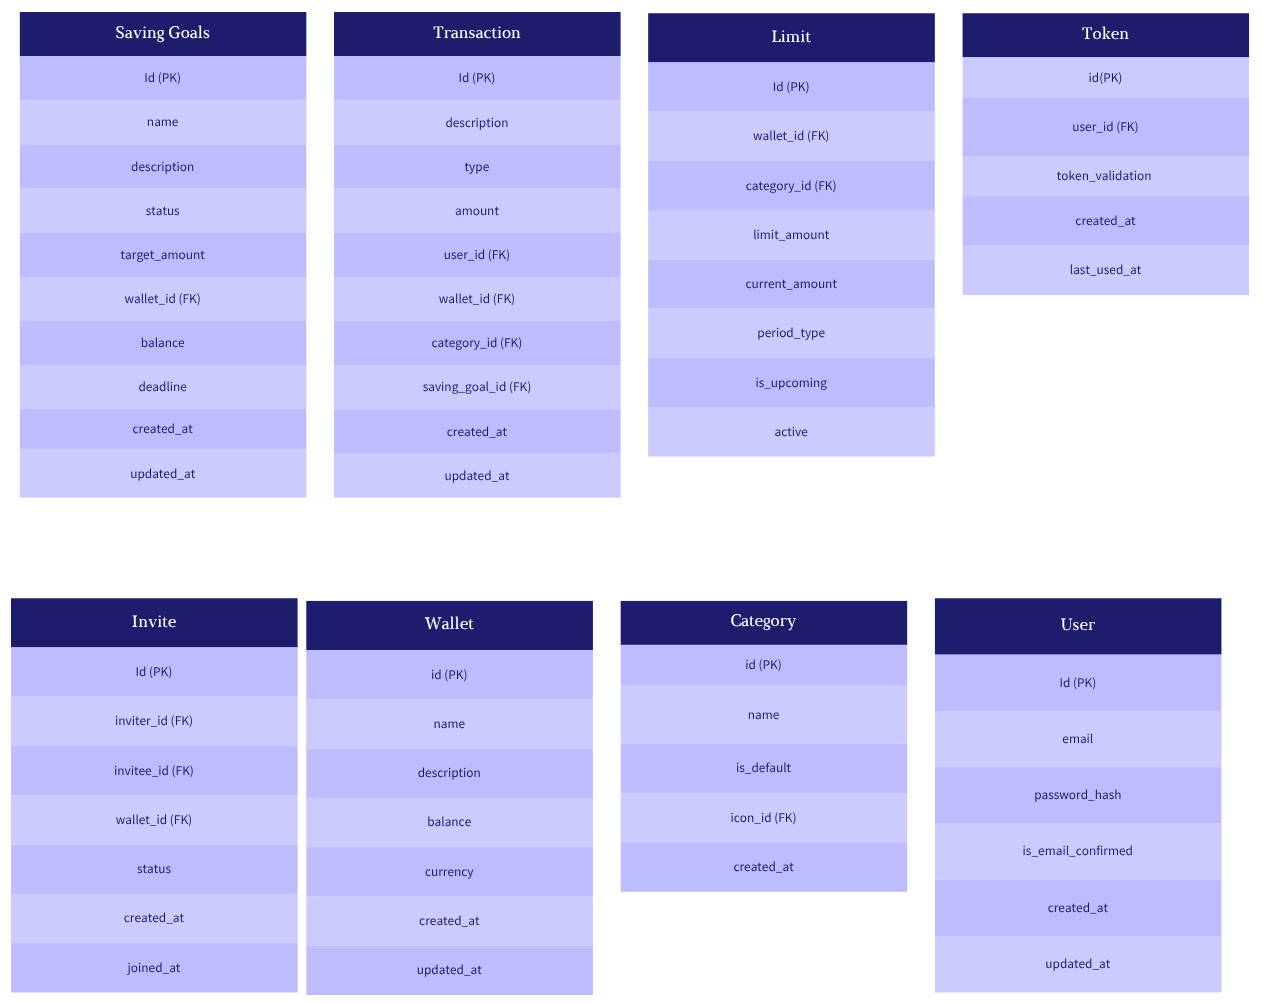
\includegraphics[width=1\textwidth]{./img/table_1.png}
        \caption{Atributte Table 1}
        \label{fig:sub:table1}
    \end{subfigure}


    \begin{subfigure}[b]{\textwidth}
        \centering
        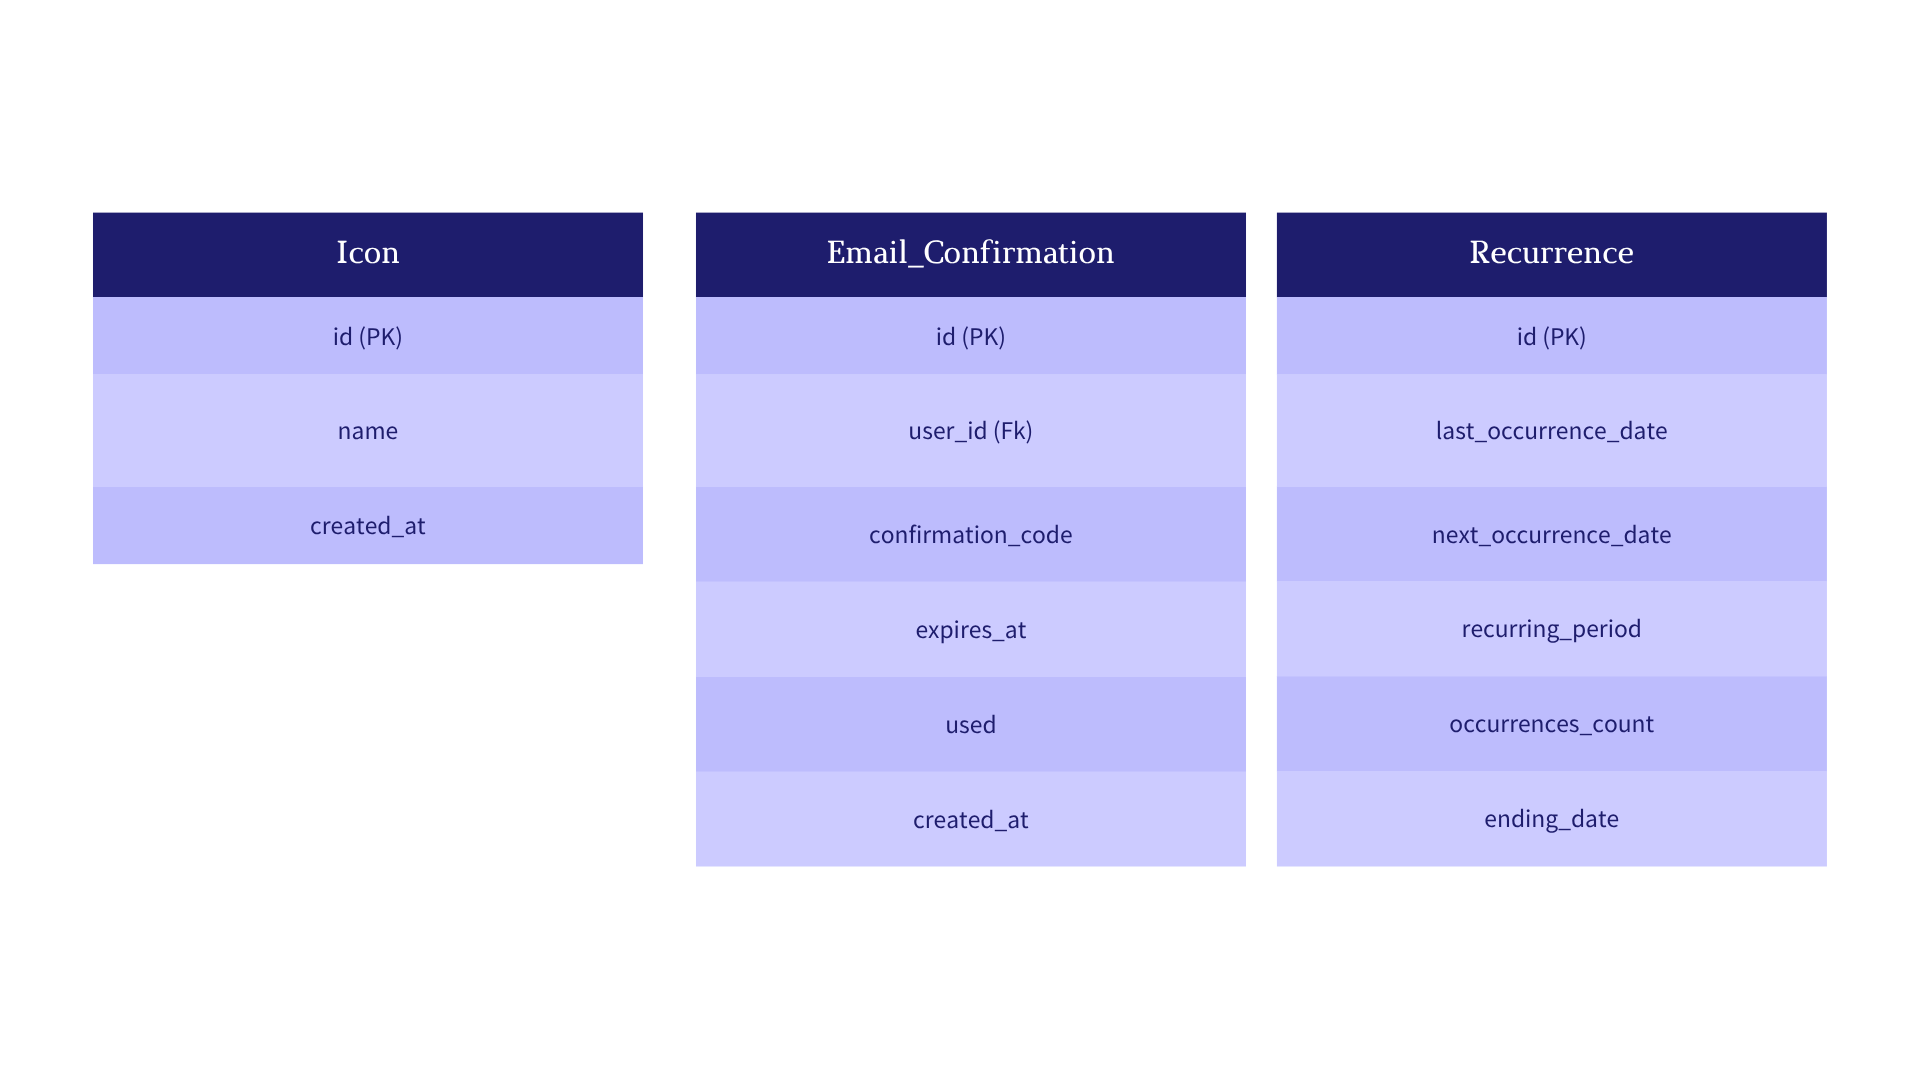
\includegraphics[width=1\textwidth]{./img/table_2.png}
        \caption{Atributte Table 2}
        \label{fig:sub:table2}
    \end{subfigure}
    \caption{Attributes of every entity in the database}
    \label{fig:database_tables}
\end{figure}

The relational model was designed to support the functional and structural needs of a marketplace platform. Each entity and its attributes were carefully selected to reflect real-world concepts such as users, wallets, transactions, goals, and access control. Below is an intuitive justification for the key design decisions:
\begin{itemize}
    \item \textbf{USER}: Represents individual users of the platform. Attributes like email, username, and password\_hash are essential for authentication. The flags is\_email\_confirmed and timestamps help with account lifecycle management.

    \item \textbf{WALLET}: A wallet groups financial data and can be shared among multiple users. It includes balance, currency, and optional description, supporting both individual and group financial tracking.

    \item \textbf{USER\_WALLET}: Models a many-to-many relationship between users and wallets, with an is\_owner flag to distinguish between owners and invited participants.

    \item \textbf{INVITE}: Captures the invitation flow when users are invited to join wallets. The status and joined\_at fields allow tracking of invitation state over time.

    \item \textbf{TOKEN}: Stores session or login tokens for users. Includes created\_at and last\_used\_at to support expiration and activity tracking, promoting secure authentication.

    \item \textbf{EMAIL\_CONFIRMATION}: Used during account creation, storing a unique code, its expiration, and usage status for email verification workflows.

    \item \textbf{ICON} and \textbf{CATEGORY}: Categories help classify transactions (e.g., Groceries, Rent). Each category may be linked to an icon for UI clarity, and the is\_default flag identifies system-defined options. Color and icon references support user personalization.

    \item \textbf{WALLET\_CATEGORY}: Allows each wallet to customize which categories are available, ensuring separation between shared and personal classification systems.

    \item \textbf{TRANSACTION}: Central to the platform, each transaction records amount, type (e.g., income, expense, save), associated wallet, user, category, and optionally links to a saving goal or recurrence rule.

    \item \textbf{SAVING\_GOALS}: Lets users define goals like \emph{Vacation Fund} with a target\_amount, balance, deadline, and status. Tied to a wallet to allow shared or personal goals.

    \item \textbf{RECURRENCE}: Abstracts recurring transaction logic with fields such as recurring\_period, next\_occurrence\_date, and ocurrences\_count. Linked to TRANSACTION when applicable.

    \item \textbf{LIMIT}: Enables setting monthly or weekly spending limits per wallet (and optionally per category). It tracks the current\_amount spent and the limit\_amount, helping users stay on budget.
\end{itemize}

\section{Triggers and Functions}
To help us have less code and unnecessary logic on the API we decided to make some automatic actions on the database using triggers and functions. This helped us to have a more efficient and cleaner code, and also not have to worry about specific logic.

\subsection{Trigger for updating the limit amount when transaction is created}
This trigger is responsible for automatically updating spending limits when a new transaction is recorded in the system. Our application allows users to create spending limits that establish boundaries on the amount of money they can spend, either within specific categories or across all categories (total limit).

When a transaction is created, the trigger performs the following actions:
\begin{itemize}
    \item Checks if there exists any limit associated with the transaction's category and/or a total spending limit.
    \item If a limit exists, verifies whether it has expired. If expired, the trigger marks that limit as inactive and creates a new one. This verification serves as a failsafe, though it should rarely be needed since scheduled tasks regularly check for and handle expired limits.
    \item Updates the current accumulated amount of the relevant limits to reflect the new transaction.
\end{itemize}

For example, if a user has set a monthly limit of \$500 for \emph{Food} category and makes a new purchase of \$50 in that category, the trigger automatically increases the current accumulated amount for that limit from, say, \$200 to \$250, ensuring the user can always see how much of their limit they've used.

\sloppy
Figure~\ref{fig:create_limit_trigger} illustrates this process, showing how the trigger affects the spending limits when a new expense transaction is created. The diagram shows the state of the category limit and total limit before and after the transaction is recorded in the system.

\begin{figure}[H]
    \centering
    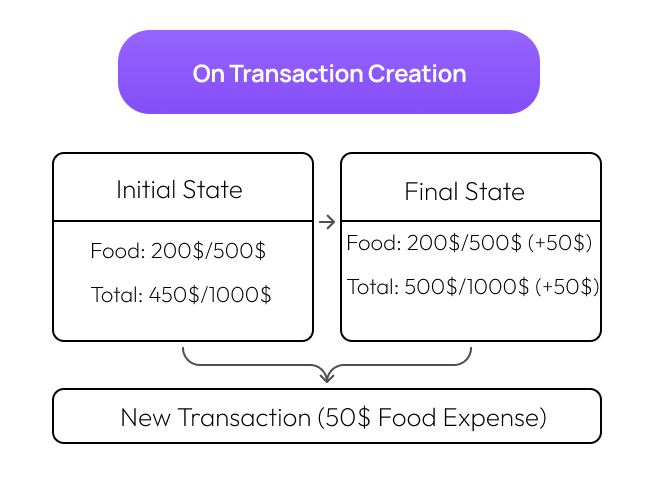
\includegraphics[width=8cm]{img/trigger_on_transaction_create.png}
    \caption{Process of updating limits when a new expense transaction is created.}
    \label{fig:create_limit_trigger}
\end{figure}

\subsection{Trigger for updating the limit amount when transaction is updated}
This trigger manages the recalculation of spending limits when an existing transaction is modified. It uses a straightforward approach to ensure limits remain accurate regardless of what aspects of the transaction were changed.

When a transaction is updated, the trigger executes this process:
\begin{itemize}
    \item First, if the original transaction was an expense, it completely removes the transaction's impact from both the total limit and the category-specific limit.
    \item Then, if the updated transaction is still an expense, it adds the new transaction value to both the total limit and the new category's limit.
\end{itemize}

This two-step approach effectively treats the update as a deletion of the old transaction followed by an insertion of the new one. It handles all possible modification scenarios including:
\begin{itemize}
    \item Changes to the transaction amount
    \item Changes to the transaction category
    \item Changes to the transaction type (from expense to income or vice versa)
    \item Any combination of the above changes
\end{itemize}

For example, if a user changes a \$75 \emph{Entertainment} expense to a \$100 \emph{Dining} expense, the trigger first subtracts \$75 from the \emph{Entertainment} limit and the total limit, then adds \$100 to the \emph{Dining} limit and the total limit.

Figure~\ref{fig:update_limit_trigger} illustrates this update process, showing how the trigger manages changes to limits when a transaction is modified. The diagram demonstrates the complete flow of the operation, from the initial state to the final state, including all intermediate steps of removing and adding values.

\begin{figure}[H]
    \centering
    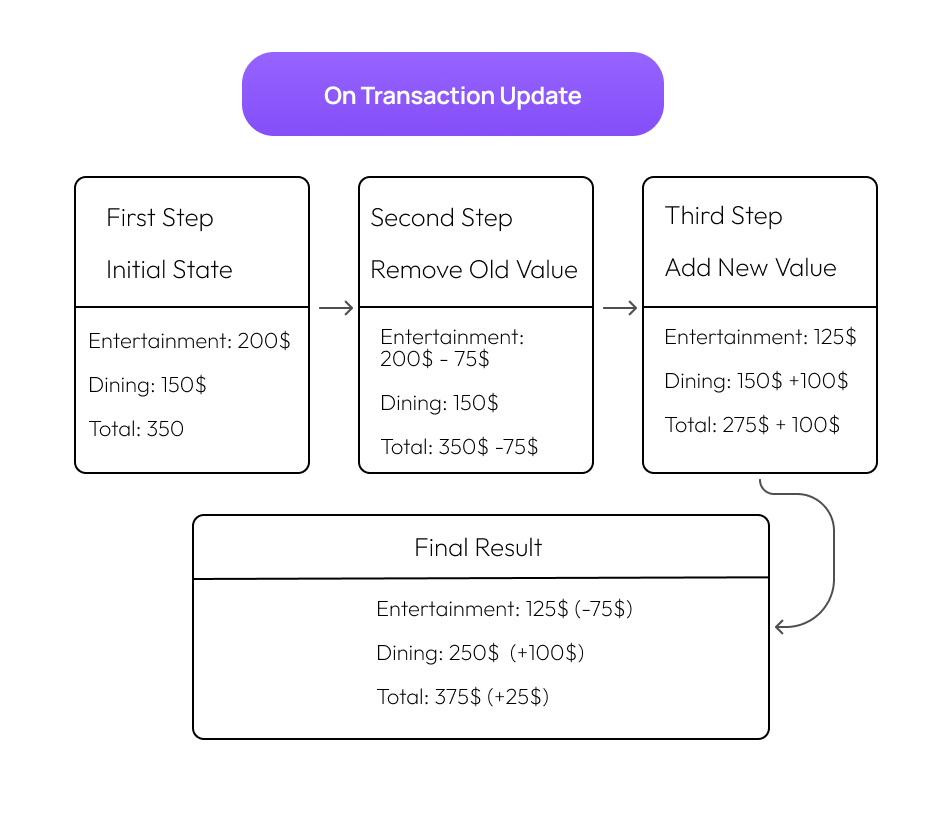
\includegraphics[width=8cm]{img/trigger_on_transaction_update.png}
    \caption{Process of updating limits when a transaction is edited to other category with a diferent amount}
    \label{fig:update_limit_trigger}
\end{figure}


\subsection{Trigger for updating the limit amount when transaction is deleted}
This trigger manages the adjustment of spending limits when a transaction is removed from the system. Deleting transactions requires recalculating the associated spending limits to maintain accurate budget tracking.

When a transaction is deleted, the trigger performs these operations:
\begin{itemize}
    \sloppy
    \item Identifies which spending limits are affected by the deleted transaction (category-specific and/or total limits).
    \item Verifies that these limits are still active and not expired.
    \item Decreases the accumulated amount of each affected limit by the transaction amount, effectively \emph{giving back} the spent amount to the user's available budget.
    \item Ensures that the limit's current amount doesn't fall below zero after the adjustment.
\end{itemize}

For instance, if a user mistakenly recorded a \$120 grocery purchase and later deletes it, the trigger automatically reduces the accumulated amount in their \emph{Groceries} limit by \$120. If their limit was previously at \$350 out of \$500, it would now show \$230, correctly reflecting that they have more available budget than previously indicated.

Figure~\ref{fig:delete_limit_trigger} illustrates this process, showing how the trigger adjusts the spending limits when a transaction is deleted. The diagram demonstrates how the removal of a transaction leads to the corresponding reduction in the accumulated amounts for both the category-specific limit and the total spending limit.

\begin{figure}[H]
    \centering
    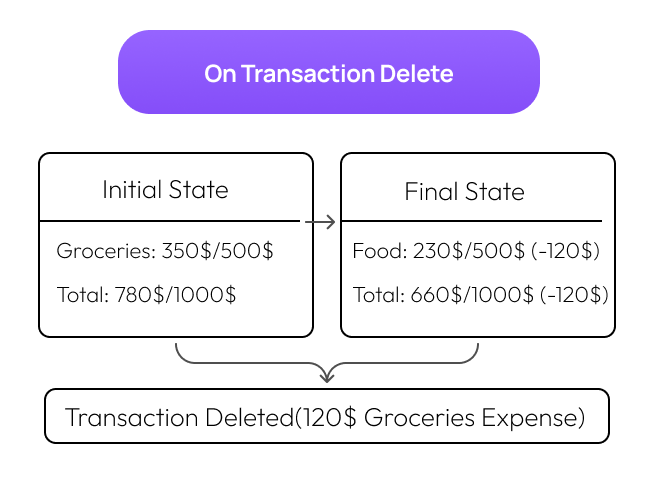
\includegraphics[width=9cm]{img/trigger_on_transaction_delete.png}
    \caption{Process of updating limits when a transaction is deleted}
    \label{fig:delete_limit_trigger}
\end{figure}

\subsection{Trigger for adding default categories to a new wallet}
This trigger simplifies the wallet setup process by automatically associating newly created wallets with a predefined set of categories. This ensures users can immediately begin tracking their expenses without having to manually configure categories.

For example, when a user creates a new wallet, it will automatically be configured with the default categories like \emph{Food}, \emph{Transportation}, \emph{Housing}, \emph{Entertainment}, and \emph{Utilities}. This means the user can immediately begin categorizing their transactions without any additional setup.

This automatic initialization improves the user experience by reducing the initial configuration required and ensuring consistency across wallet setups. Users can still customize their categories later by adding new ones that make more sense for their specific needs.
